\documentclass[a4paper,11pt]{article}
\usepackage[big]{layaureo}
\usepackage[T1]{fontenc}
\usepackage[utf8]{inputenc}
%\usepackage[italian]{babel}
\usepackage{fancyhdr}
\usepackage{textcomp}
\usepackage{amsmath}
\usepackage{amssymb}
\usepackage{mathtools}
\usepackage{multirow}
\usepackage{caption}
  \captionsetup{format=plain,labelfont=bf,textfont=it, font=small}
\usepackage{subcaption}
  \captionsetup[sub]{position=top}
  \captionsetup[sub]{font=footnotesize}
  \captionsetup[sub]{labelfont={bf,sc}}
  \captionsetup[sub]{format=hang}
\usepackage{booktabs}
\usepackage{tabularx}
\usepackage{float}
\usepackage{wrapfig}
\usepackage{comment}
\usepackage[dvipsnames]{xcolor}
\usepackage{listings}

\definecolor{light-gray}{gray}{.95}
\lstset{frame=none,
  aboveskip=3mm,
  belowskip=3mm,
  showstringspaces=false,
  columns=fullflexible,
  keepspaces=true,
  numbers=none,
  basicstyle={\footnotesize\ttfamily},
  numberstyle=\tiny\color{gray},
  keywordstyle=\color{NavyBlue},
  stringstyle=\color{Orange},
  commentstyle=\color{OliveGreen},
  breaklines=true,
  breakatwhitespace=true,
  tabsize=4,
  backgroundcolor=\color{light-gray}
}

\title{Neural Network and Deep Learning \\ Homework 2}
\author{Federico Agostini}
\date{}

\begin{document}

\maketitle

\section{Introduction}
In this exercise a feed-forward neural network implemented with \texttt{Pytorch} is used to learn the MNIST dataset of handwritten digits.

The number of neurons in each of the two hidden layers has beeen selected after a search procedure with a cross validation tecnique.

\section{Model selection and parameters search}
The dataset consists on 60000 images of handwritten digits; it has been divided into training (80\%) and test set (20\%). The optimization of the hyperparameters of the network is done using a cross validation procedure using the training set. In particular, a 5-fold CV is implemented with 1000 epochs per training. The error associated is the mean accuracy, that is the fraction of correct classified patterns.

The best model is chosen as the one with the smallest validation error (calculated as the mean of the 5 errors obtained during CV). After that, it is retrained using the whole training set and the final mean accuracy is calculated over the test set.

The architecture chosen for the task is a neural network with two hidden layer and ReLU as activation function; the optimization procedure tunes the number of neurons in each layer and the best optimizer between \texttt{Adam} and \texttt{RMSprop}. In particular, for the first hidden layer 10 random values in the range $[100, 500]$, while for the second one the number is in the list \texttt{[x**2 for x in range(11,21)]}. The ranges are chosen looking at example of the same problem, while the choice of squared number for the second layer is for visualize graphically the receptive fileds of the output neurons.

Tab.~\ref{tab:ParamSearch} reports the best solution obtained after CV training. Due to large time needed to perform the training (200 total combination of parameters), no other choice of the activation function or number of layer has been implemented.

\begin{table}[hp]
    \centering
    \caption{Best results obtained after the hyperparameters search.}
    \label{tab:ParamSearch}
    \begin{tabular}{cccr}
        \toprule
         $1^{st}$ hidden layer &  $2^{nd}$ hidden layer & Optimizer &   Val\_Loss \\
        \midrule
         280 &  121 &      Adam &   0.030274 \\
         398 &  361 &      Adam &   0.031036 \\
         398 &  225 &      Adam &   0.032040 \\
         280 &  289 &      Adam &   0.032480 \\
         173 &  400 &      Adam &   0.032498 \\
         \bottomrule
    \end{tabular}
\end{table}

\section{Final model}
The final model is obtained using \texttt{Adam} as optimizer and has 280 neurons in the first hidden layer and 121 in the second one.

The whole training set is then used to train this model before making predictions on the test set. The training procedure is done with 3000 epochs, but overfitting occurs, as shown in Fig.~\ref{fig:loss}. So the network is trained again from scratch, but stopping early at 350 epochs. The final mean accuracy evaluated on the test set results to be 97.2\%.

\begin{figure}[hp]
    \centering
    \caption{Training and test loss for the best model}
    \label{fig:loss}
    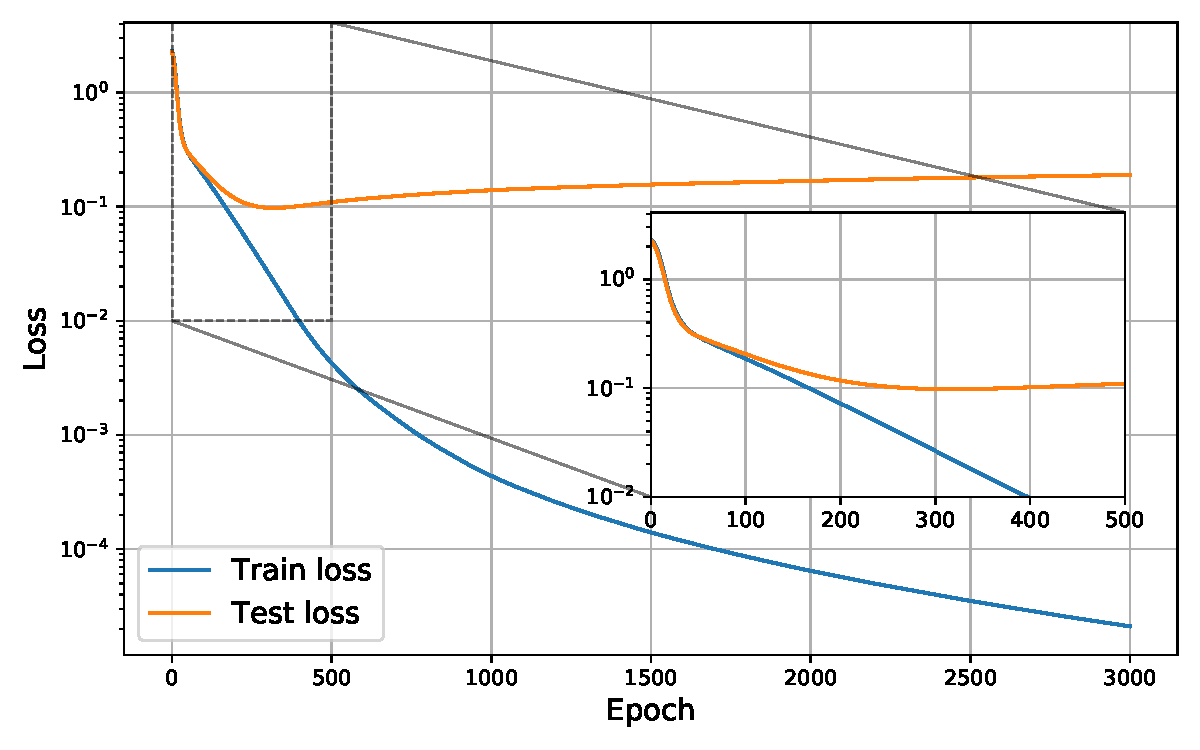
\includegraphics[width=.75\linewidth]{../Figure/Loss.pdf}
\end{figure}

Fig.~\ref{fig:Confusion} shows the confusion matrix of true/predicted labels on the test set. It can be noticed that except for the number 4 being confused with 9 (that occurs with 2.3\% probability), all the errors appears with probability of less than 0.01.

Fig.~\ref{fig:Receptive} displays receptive fields of the 10 output neurons, while Fig.~\ref{fig:Weights} shows the weights distribution of the three layers of the neural network.

\begin{figure}[hp]
    \centering
    \caption{Confusion matrix of the best model over the test set; rows are normalized. The second figure is done removing the elements in the diagonal (e.g. correct classifications), in order to get a clearer view over misclassification errors.}
    \label{fig:Confusion}
    \begin{subfigure}[t]{.75\linewidth}
        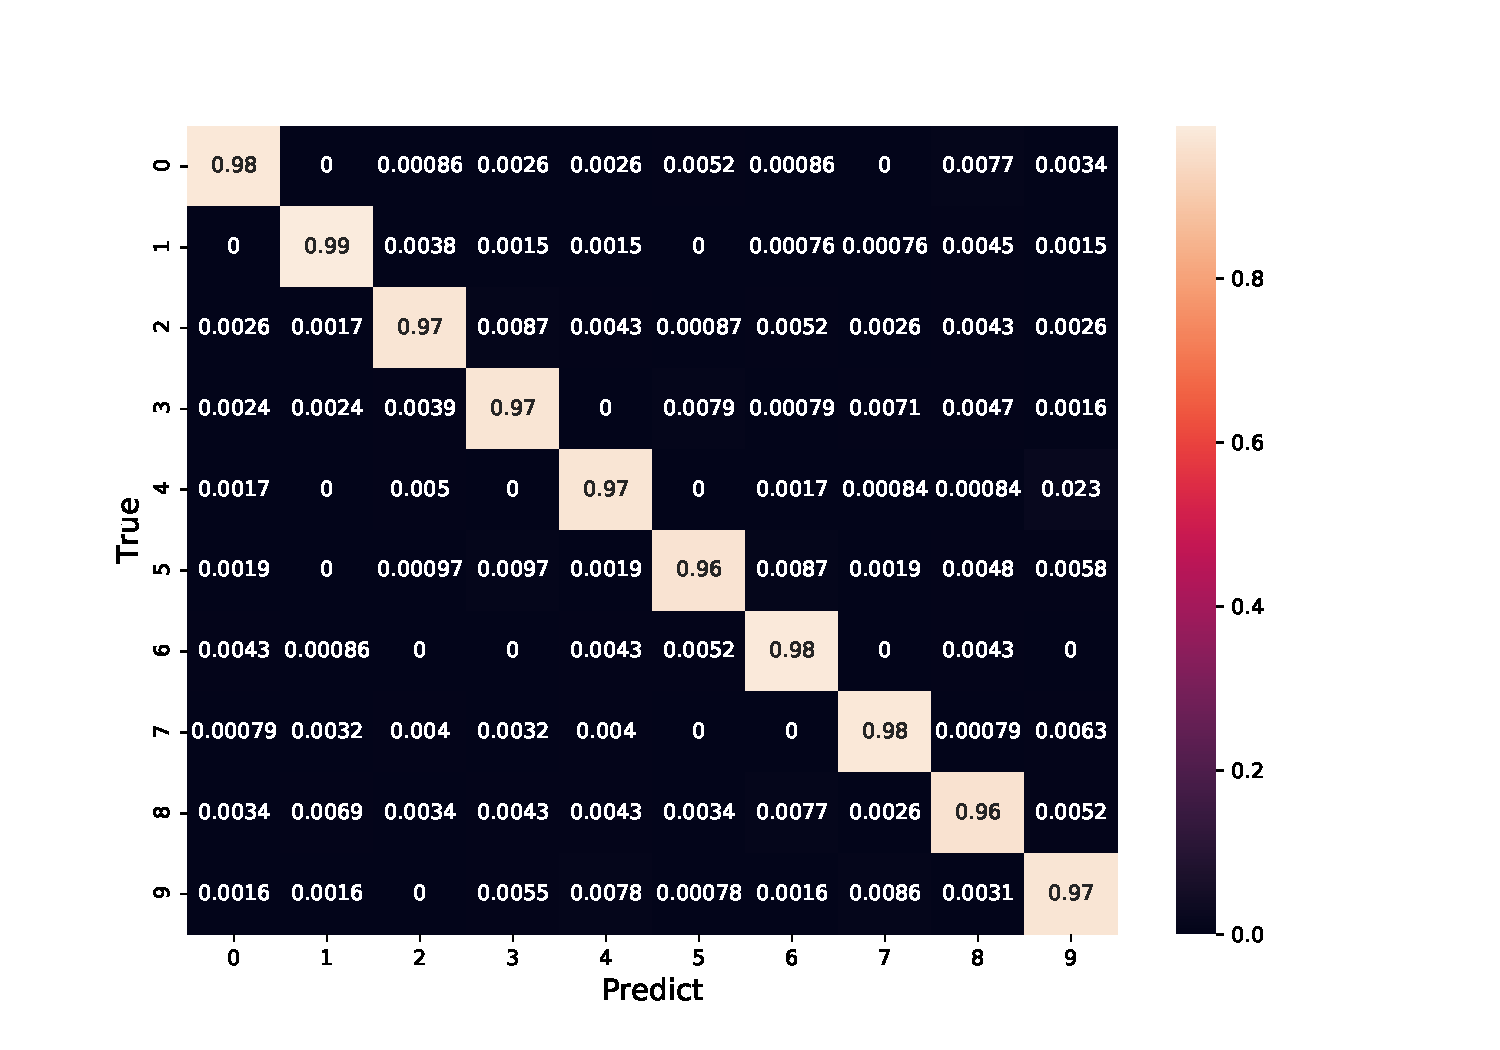
\includegraphics[width=\linewidth]{../Figure/Confusion_complete}
        \caption{Complete confusion matrix.}
    \end{subfigure}
    \begin{subfigure}[t]{.75\linewidth}
        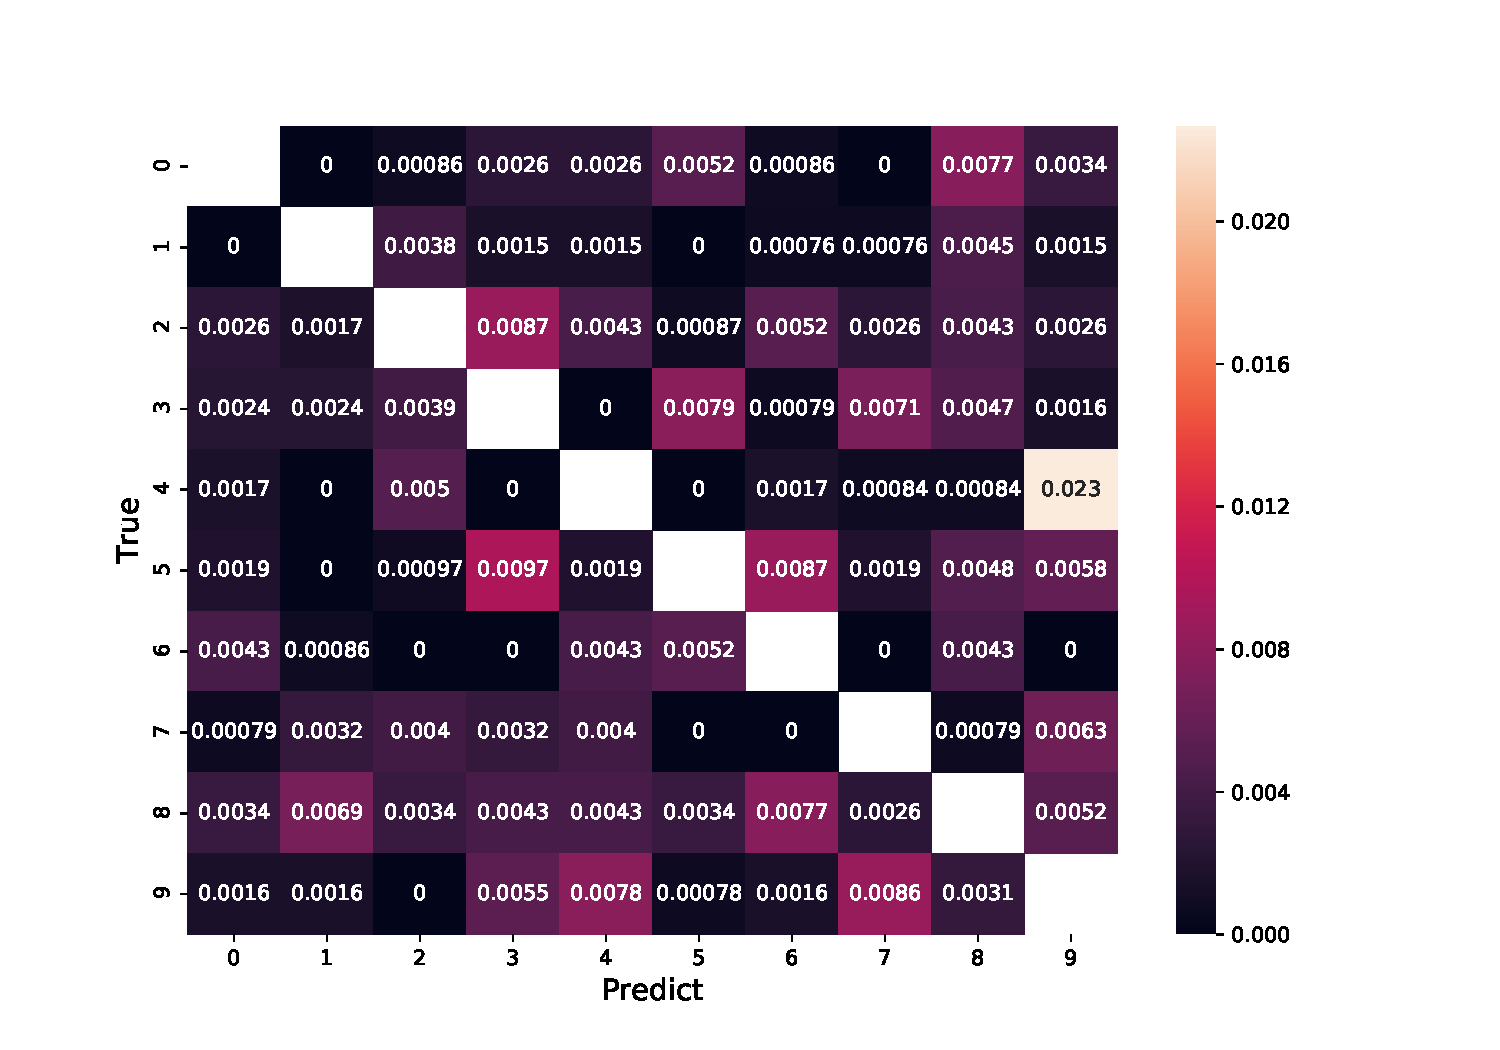
\includegraphics[width=\linewidth]{../Figure/Confusion_errors}
        \caption{Confusion matrix without correct classifications.}
    \end{subfigure}
\end{figure}

\begin{figure}[hp]
    \centering
    \caption{Receptive field of the output neurons.}
    \label{fig:Receptive}
    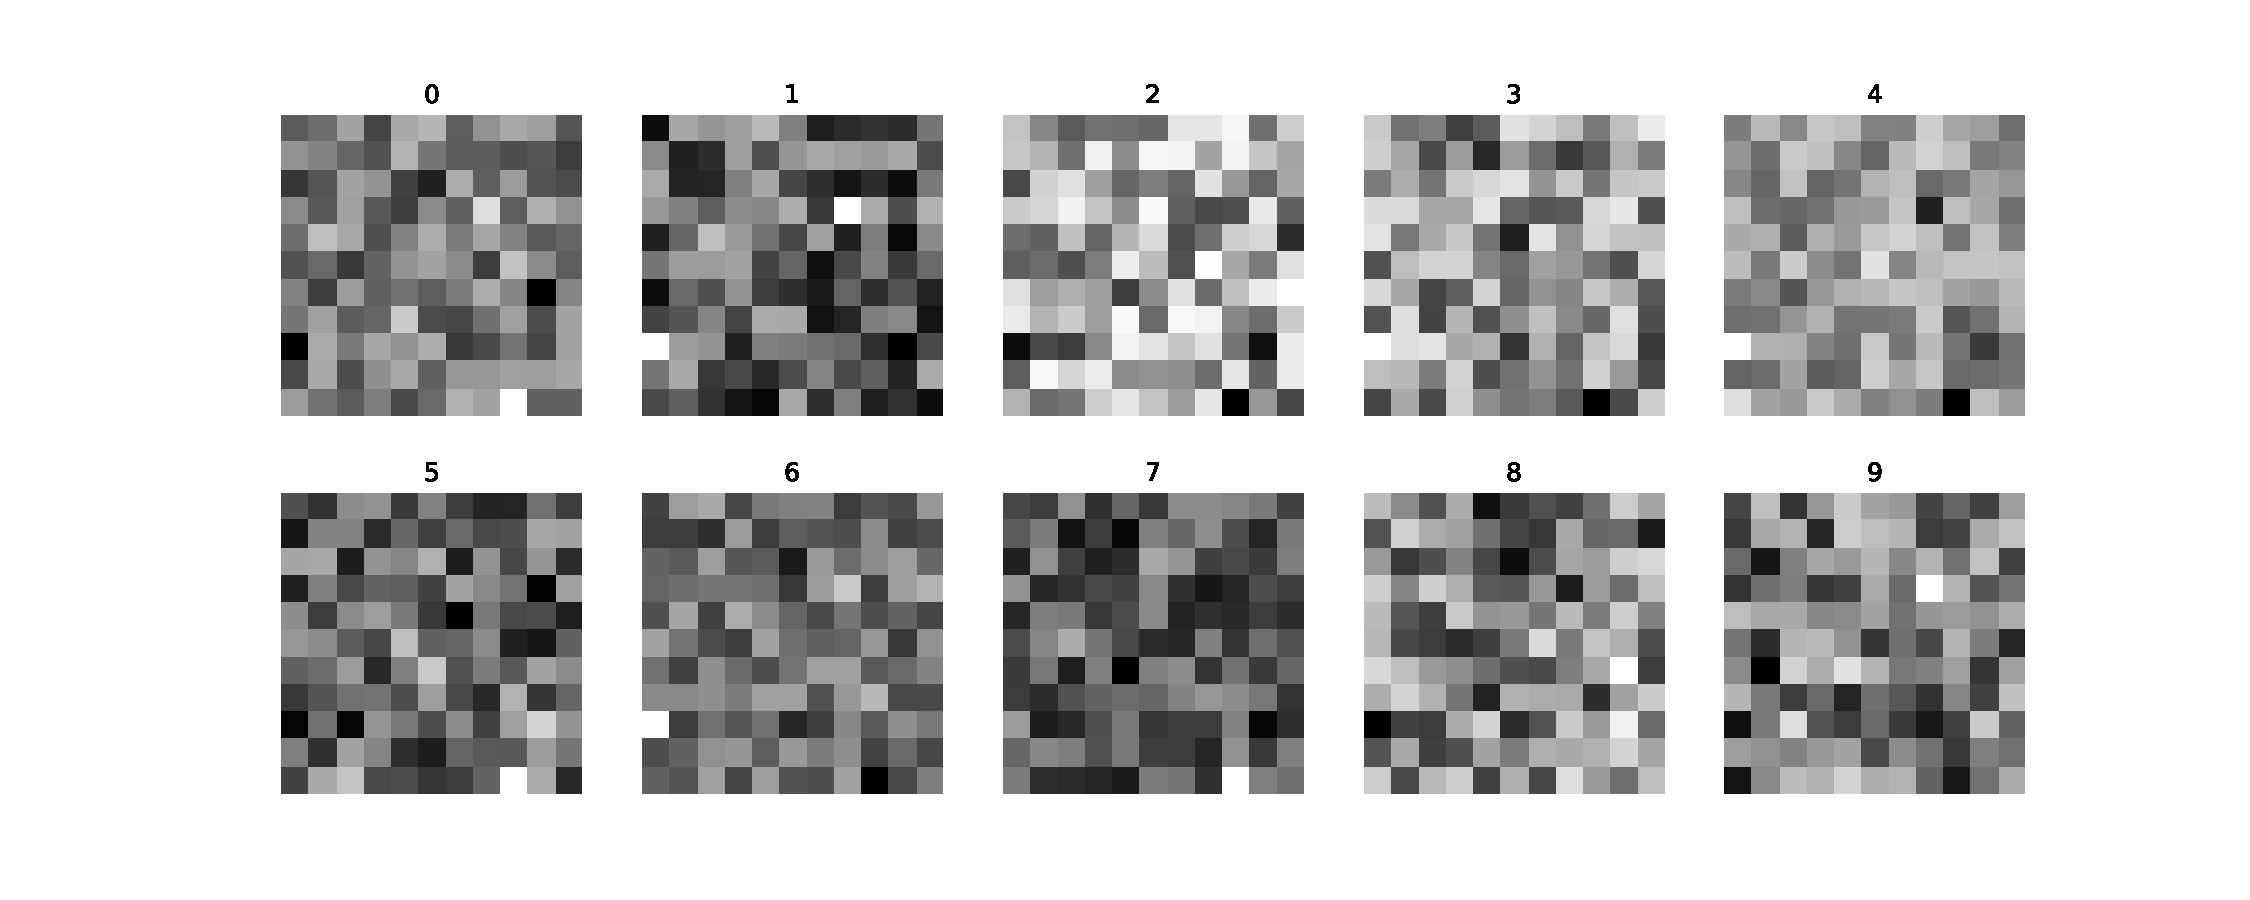
\includegraphics[width=\linewidth]{../Figure/ReceptiveField.pdf}
\end{figure}

\begin{figure}[hp]
    \centering
    \caption{Weights distribution of the neurons of the layers of the neural network.}
    \label{fig:Weights}
    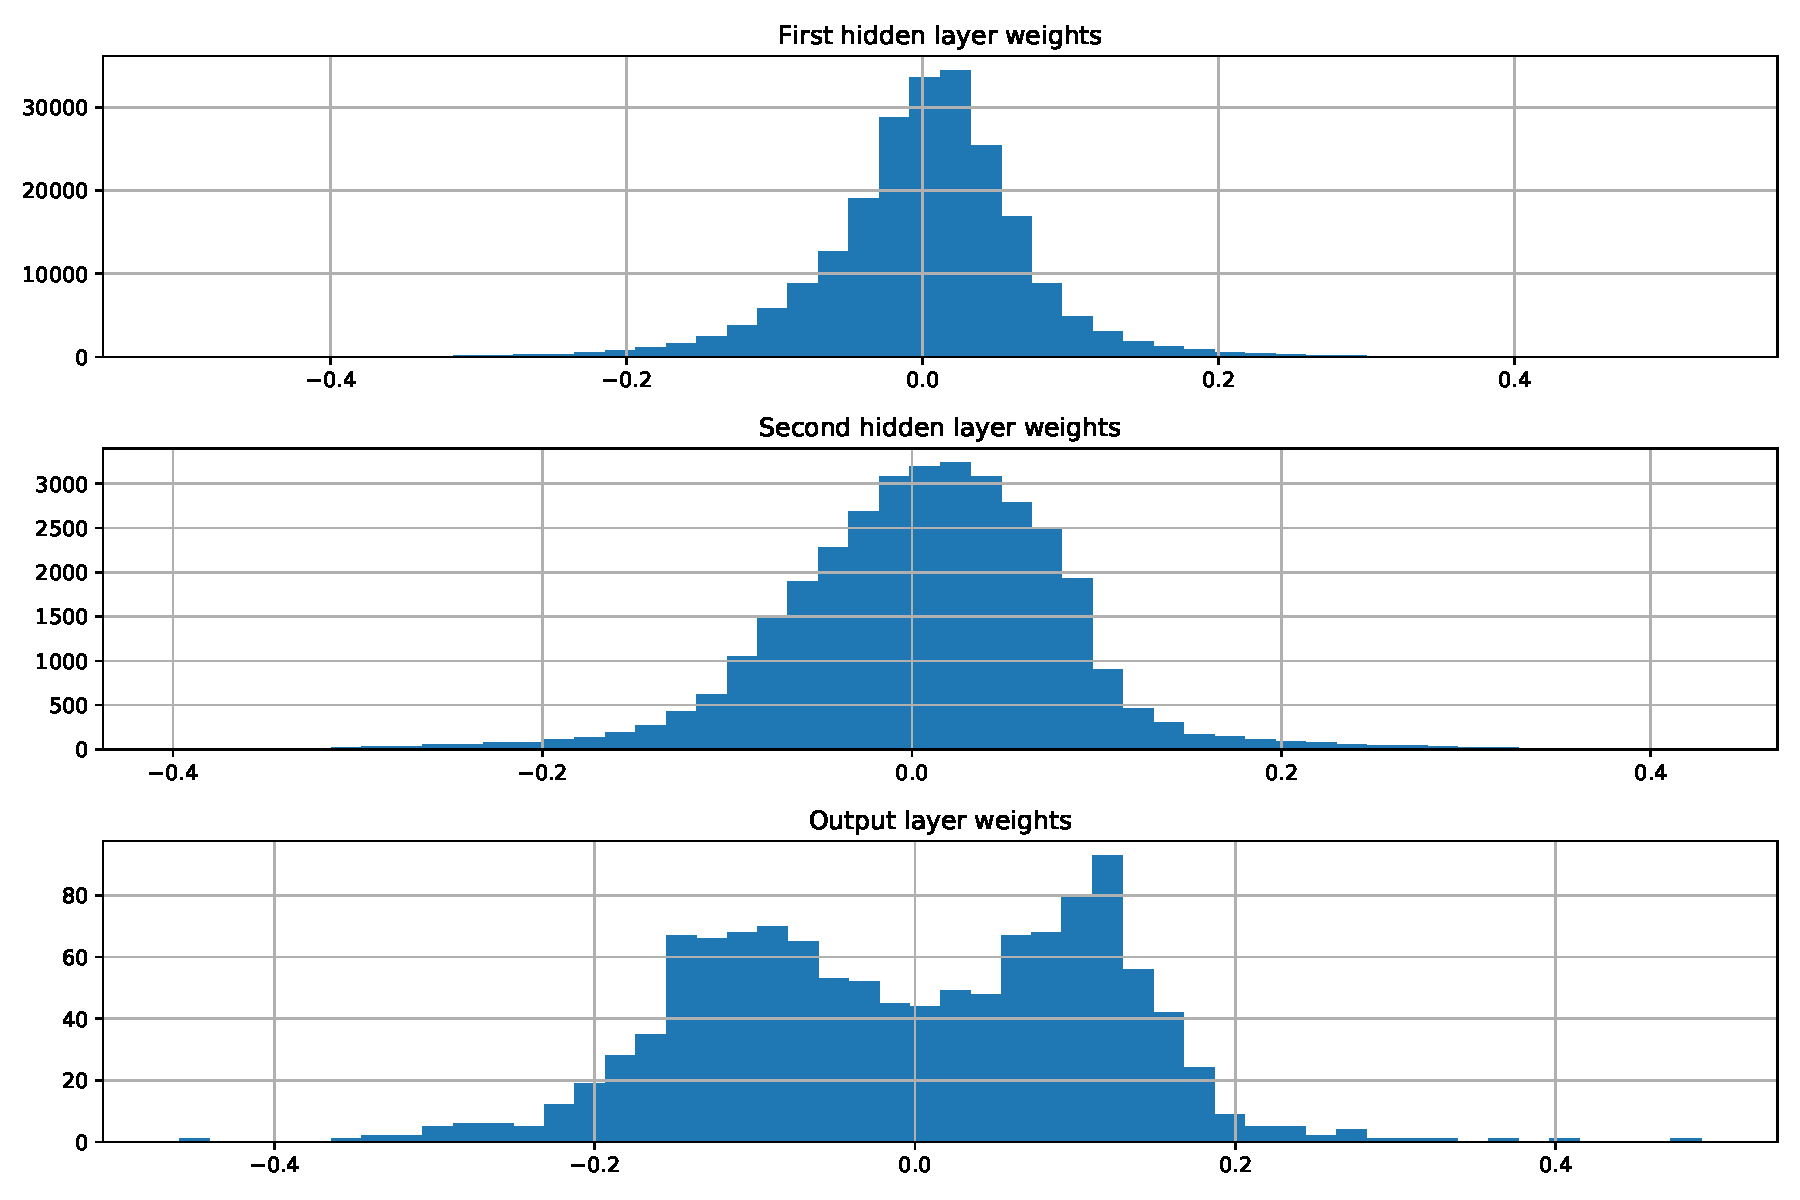
\includegraphics[width=.75\linewidth]{../Figure/Weights.pdf}
\end{figure}

\end{document}
